%%%%%%%%%%%%%%%%%%%%%%%%%%%%%%%%%%%%%%%%%
% 
% LaTeX Template
% Version 3.1 (25/3/14)
%
%%%%%%%%%%%%%%%%%%%%%%%%%%%%%%%%%%%%%%%%%

%----------------------------------------------------------------------------------------
%	PACKAGES AND DOCUMENT CONFIGURATIONS
%----------------------------------------------------------------------------------------

\documentclass[12pt, a4 paper]{article}

\usepackage{tikz}
%\usepackage[top=2cm, bottom=2cm, outer=0cm, inner=0cm]{geometry}
\usepackage{graphicx} % Required for the inclusion of images
\usepackage{multicol} % Required for multicolumns
\usepackage{setspace} % Required for line spacing
\setlength\parindent{0pt} % Removes all indentation from paragraphs
\setlength{\columnseprule}{0.4pt} % Adds vertical line between multicolumns
\usepackage{multirow} % Required for multirows
\usepackage{booktabs} % For prettier tables
\usepackage{xcolor}
%\usepackage{tabularx}
%\renewcommand{\rmdefault}{ptm}

%\usepackage{helvet}

\usepackage{times} % Uncomment to use the Times New Roman font

%----------------------------------------------------------------------------------------
%	DOCUMENT INFORMATION
%----------------------------------------------------------------------------------------

\begin{document}

\tikz[remember picture,overlay] \node[opacity=0.3,inner sep=0pt] at (current page.center){
\includegraphics[width=\paperwidth,height=\paperheight]{placeholder.jpg}};

\clearpage

%\font\myfont=cmr12 at 35pt
%\title{\myfont  Event Name} % Write Event name here
%\author{}
%\date{\vspace{-10ex}}

%\maketitle % Insert the title, author and date
\setstretch{1.5}

\tikz[remember picture,overlay] \node[opacity=0.8,inner sep=0pt] at (current page.center){
\includegraphics[width=\paperwidth,height=\paperheight]{Border48-A4--Arvin61r58.png}};
%\tikz[remember picture,overlay] \node[opacity=0.5,inner sep=0pt] at (current page.center){
\includegraphics[width=\paperwidth,height=\paperheight]{color-2174049__340.png}};

\begin{center}
\Huge \bfseries \ttfamily Event Name
\end{center}

\begin{center}
\large A Short Description
\end{center}

\begin{center}
\begin{multicols}{2}
\begin{tabular}{l r}
Date: & 00/00/0000\\ % Date the event was held
Time: & X pm to Y pm \\ % Time of event 
\end{tabular}
\columnbreak
\begin{tabular}{l r}
Venue: & Dummy \\ % Venue of event
Total Attendance: & Number \\ % Number of participants
\end{tabular}
\end{multicols}


\begin{LARGE}
Name of rounds in this single line
\end{LARGE}

\begin{Large}
\begin{multicols}{2}
Some paragraph
\columnbreak

\includegraphics[width=\linewidth]{placeholder.jpg}
  %\caption{A boat.}
  %\label{fig:boat1}
\end{multicols}

\begin{multicols}{2}


\includegraphics[width=\linewidth]{placeholder.jpg}

\columnbreak
Some paragraph
\end{multicols}

\newpage 

\tikz[remember picture,overlay] \node[opacity=0.8,inner sep=0pt] at (current page.center){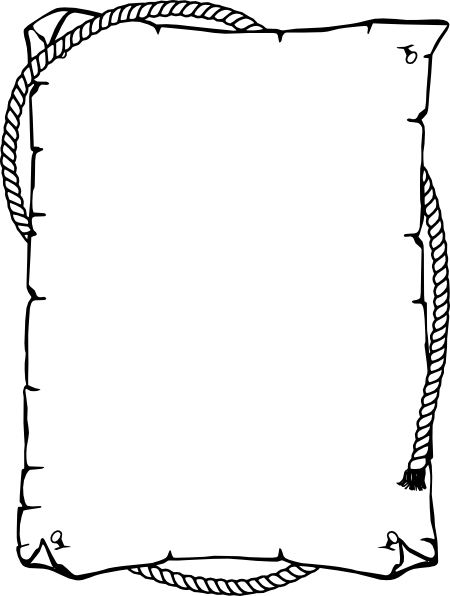
\includegraphics[width=\paperwidth,height=\paperheight]{5TRrp44jc.png}};
%\tikz[remember picture,overlay] \node[opacity=0.8,inner sep=0pt] at (current page.center){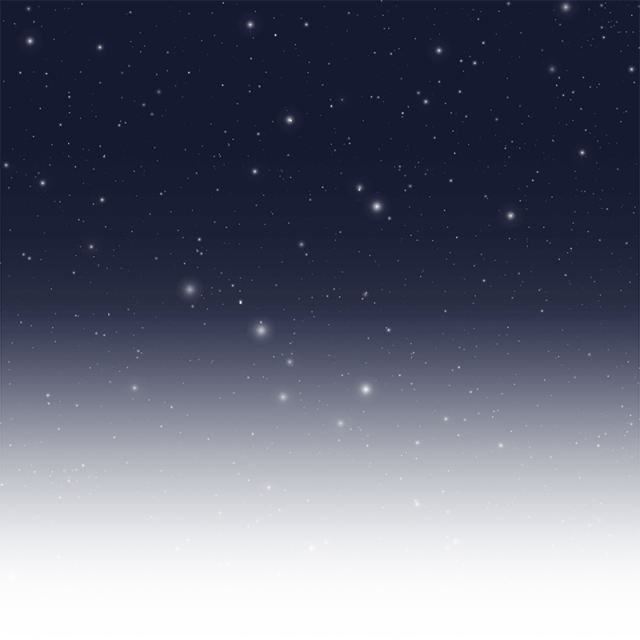
\includegraphics[width=\paperwidth,height=\paperheight]{md_5b0912b7c0870.png}};

\begin{multicols}{2}
Some paragraph
\columnbreak

\includegraphics[width=\linewidth]{placeholder.jpg}
  
\end{multicols}

\begin{multicols}{2}

\includegraphics[width=\linewidth]{placeholder.jpg}

\columnbreak
Some paragraph
  
\end{multicols} 

\begin{multicols}{2}
Some paragraph

\columnbreak

\includegraphics[width=\linewidth]{placeholder.jpg}
  
\end{multicols} 

\begin{multicols}{2}

\includegraphics[width=\linewidth]{placeholder.jpg}

\columnbreak
Some paragraph
  
\end{multicols} 

\end{Large} 
\end{center}

\newpage 

\tikz[remember picture,overlay] \node[opacity=0.8, inner sep=0pt] at (current page.center){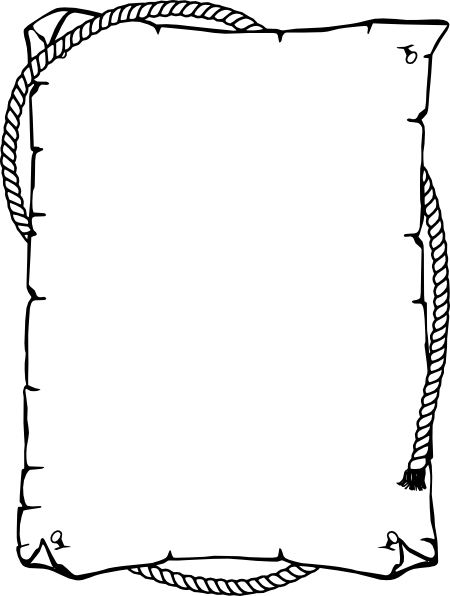
\includegraphics[width=\paperwidth,height=\paperheight]{5TRrp44jc.png}};
\tikz[remember picture,overlay] \node[opacity=0.8,inner sep=0pt] at (current page.center){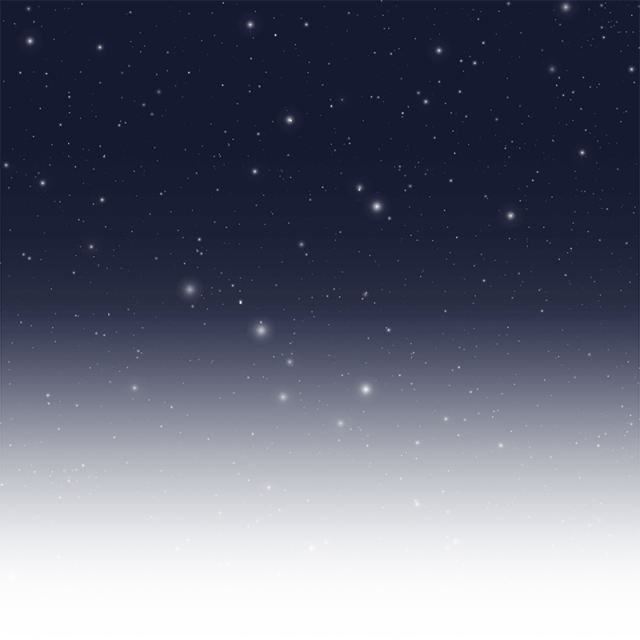
\includegraphics[width=\paperwidth,height=\paperheight]{md_5b0912b7c0870.png}};

\begin{center}
\Huge Pictures Section
\end{center}

\newpage 

\tikz[remember picture,overlay] \node[opacity=0.8,inner sep=0pt] at (current page.center){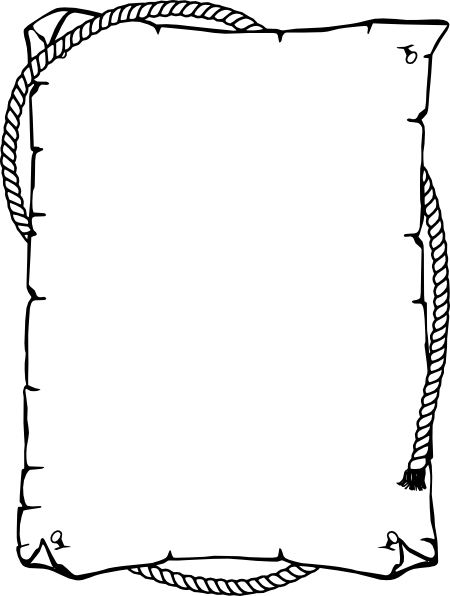
\includegraphics[width=\paperwidth,height=\paperheight]{5TRrp44jc.png}};
\tikz[remember picture,overlay] \node[opacity=0.8,inner sep=0pt] at (current page.center){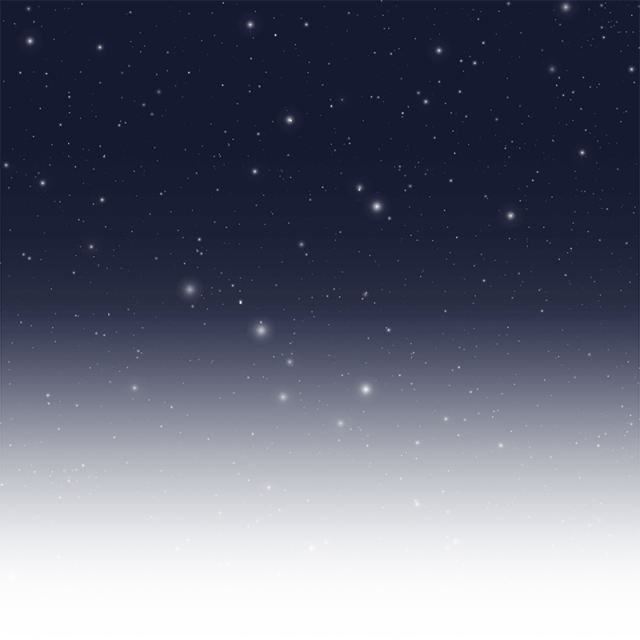
\includegraphics[width=\paperwidth,height=\paperheight]{md_5b0912b7c0870.png}};

\begin{center}
\huge Organisers list
\end{center}

\begin{table}[h!]
  \begin{center}
    \begin{tabular}{|c|c|c|c|c|c| c |} 
    \toprule % <-- Toprule here
      \textbf{S.No.} & \textbf{Name} & \textbf{Department} & \textbf{ISTE ID} &\textbf{Year/Branch} & \textbf{URN} & num \\
      \midrule % <-- Midrule here
      1 & Dummy & Dummy & Dummy & Dummy & Dummy & \\
      1 & Dummy & Dummy & Dummy & Dummy & Dummy & \\
      1 & Dummy & Dummy & Dummy & Dummy & Dummy & \\
      1 & Dummy & Dummy & Dummy & Dummy & Dummy &\\
      1 & Dummy & Dummy & Dummy & Dummy & Dummy & \\
      1 & Dummy & Dummy & Dummy & Dummy & Dummy & \\
      1 & Dummy & Dummy & Dummy & Dummy & Dummy &\\
      1 & Dummy & Dummy & Dummy & Dummy & Dummy & \\
      \bottomrule % <-- Bottomrule here
    \end{tabular}
  \end{center}
\end{table}


\begin{center}
\huge Management list
\end{center}

\begin{table}[h!]
  \begin{center}
    \begin{tabular}{|c|c|c|c|c|c|} 
    \toprule % <-- Toprule here
      \textbf{S.No.} & \textbf{Name} & \textbf{Department} & \textbf{ISTE ID} &\textbf{Year/Branch} & \textbf{URN}\\
      \midrule % <-- Midrule here
      1 & Dummy & Dummy & Dummy & Dummy & Dummy\\
      1 & Dummy & Dummy & Dummy & Dummy & Dummy \\
      1 & Dummy & Dummy & Dummy & Dummy & Dummy \\
      1 & Dummy & Dummy & Dummy & Dummy & Dummy\\
      1 & Dummy & Dummy & Dummy & Dummy & Dummy \\
      1 & Dummy & Dummy & Dummy & Dummy & Dummy \\
      1 & Dummy & Dummy & Dummy & Dummy & Dummy\\
      1 & Dummy & Dummy & Dummy & Dummy & Dummy\\
      1 & Dummy & Dummy & Dummy & Dummy & Dummy\\
      \bottomrule % <-- Bottomrule here
    \end{tabular}
  \end{center}
\end{table}

\newpage

\tikz[remember picture,overlay] \node[opacity=0.8,inner sep=0pt] at (current page.center){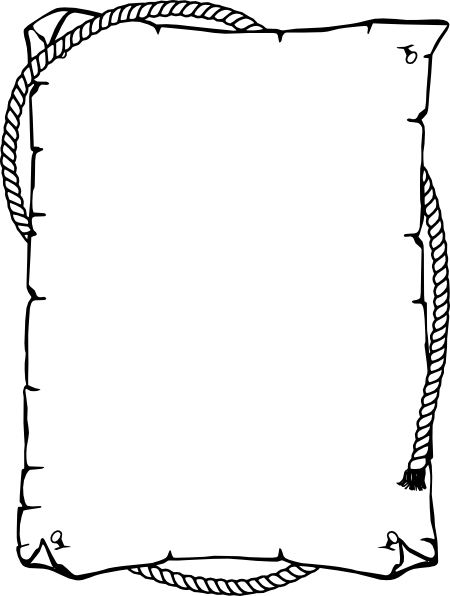
\includegraphics[width=\paperwidth,height=\paperheight]{5TRrp44jc.png}};
\tikz[remember picture,overlay] \node[opacity=0.8,inner sep=0pt] at (current page.center){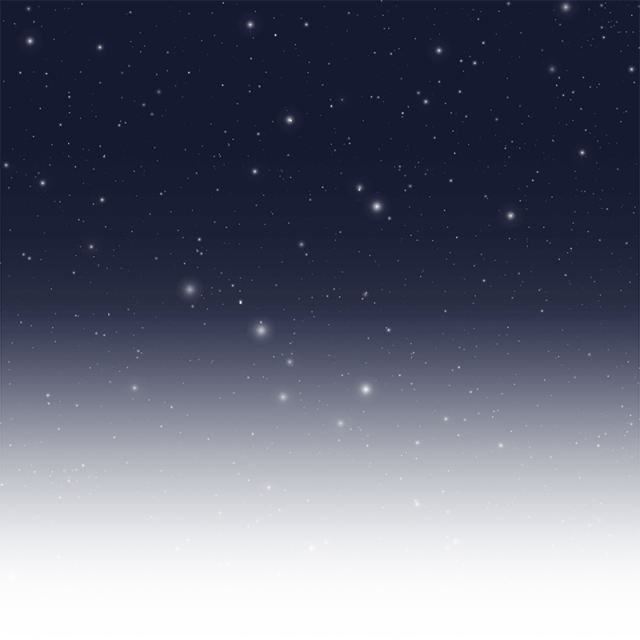
\includegraphics[width=\paperwidth,height=\paperheight]{md_5b0912b7c0870.png}};

\begin{center}
\huge Winners List
\end{center}

\begin{table}[h!]
  \begin{center}
    \begin{tabular}{|c|c|c|c|c|c|} 
    \toprule % <-- Toprule here
      \textbf{S.No.} & \textbf{Name} & \textbf{Position} & \textbf{ISTE ID} &\textbf{Year/Branch} & \textbf{URN}\\
      \midrule % <-- Midrule here
      1 & Dummy & Dummy & Dummy & Dummy & Dummy\\
      1 & Dummy & Dummy & Dummy & Dummy & Dummy\\
      1 & Dummy & Dummy & Dummy & Dummy & Dummy\\
      \bottomrule % <-- Bottomrule here
    \end{tabular}
  \end{center}
\end{table}

\begin{center}
\huge Participant list
\end{center}

\begin{table}[h!]
  \begin{center}
    \begin{tabular}{|c|c|c|c|c|c|} 
    \toprule % <-- Toprule here
      \textbf{S.No.} & \textbf{Name} & \textbf{ISTE ID} &\textbf{Year/Branch} & \textbf{URN}\\
      \midrule % <-- Midrule here
      1 & Dummy & Dummy & Dummy & Dummy \\
      1 & Dummy & Dummy & Dummy & Dummy \\
      1 & Dummy & Dummy & Dummy & Dummy  \\
      1 & Dummy & Dummy & Dummy & Dummy \\
      1 & Dummy & Dummy & Dummy & Dummy  \\
      1 & Dummy & Dummy & Dummy & Dummy  \\
      1 & Dummy & Dummy & Dummy & Dummy \\
      1 & Dummy & Dummy & Dummy & Dummy \\
      1 & Dummy & Dummy & Dummy & Dummy \\
      \bottomrule % <-- Bottomrule here
    \end{tabular}
  \end{center}
\end{table}


\end{document}